\documentclass{beamer}
\usetheme{Madrid}
\usefonttheme{default}
\useinnertheme{circles} 
\useoutertheme{infolines} 
\usecolortheme{whale}

\definecolor{i6colorscheme1}{cmyk}{0,0.7,0.839,0}
\setbeamercolor{alerted text}{fg=i6colorscheme1}

\setbeamertemplate{footline}
{
  \leavevmode%
  \hbox{%
  \begin{beamercolorbox}[wd=.2\paperwidth,ht=2.25ex,dp=1ex,center]{title in head/foot}%
    \insertframenumber{} / \inserttotalframenumber\hspace*{1ex}
  \end{beamercolorbox}%
  \begin{beamercolorbox}[wd=.6\paperwidth,ht=2.25ex,dp=1ex,center]{author in head/foot}%
    \usebeamerfont{title in head/foot}\insertshorttitle\hspace*{3em}
  \end{beamercolorbox}%
  \begin{beamercolorbox}[wd=.2\paperwidth,ht=2.25ex,dp=1ex,center]{title in head/foot}%
    \usebeamerfont{author in head/foot}\insertshortauthor
  \end{beamercolorbox}}%
  \vskip0pt%
}
\makeatletter

\usepackage{microtype}
\usepackage{fixltx2e}
\usepackage[english]{babel}

\usepackage{amsmath,amsthm, amssymb, latexsym}
\usepackage{verbatim}

\usepackage{tikz}
\usetikzlibrary{shapes, arrows, calc}

\setbeamertemplate{navigation symbols}{}
\setbeamertemplate{blocks}[rounded][shadow=true] 

%\usetheme{Boadilla}

\author[Boshen Chen]{Boshen Chen \\{\small Supervised by: Dr.\ Andrea Raith, Olga Perederieieva}}

\title[Faster Shortest Path Computation for Traffic Assignment]{Faster Shortest Path Computation for Traffic Assignment}

%\subtitle[]{}

\institute[UoA]{
    Department of Engineering Science\\
    University of Auckland\\
}

\date{}

\begin{document}

\begin{frame}[plain]
    \titlepage
    \begin{figure}
    \raggedleft
    
\includegraphics[width=5em,keepaspectratio]{img/logo}
    \end{figure}
\end{frame}

%\begin{frame}{Contents}
%    \tableofcontents
%\end{frame}

\begin{frame}{Traffic Assignment}
    \begin{itemize}
        \item transportation network with supply and demand nodes
        \item minimise travel times
        \item arcs have \alert{non-linear} travel times for capturing \alert{congestion} effects
    \end{itemize}

\end{frame}
\begin{comment}
\begin{frame}{Transportation forecasting}

    \begin{columns}
        \begin{column}{0.5\paperwidth}
            \begin{center}
                \tikzstyle{block} = [rectangle, draw, text width=10em, text centered, rounded corners, minimum height=2em]
                \tikzstyle{line} = [draw, -latex']
                \begin{tikzpicture}[node distance=4em]
                    \pause

                    \node [block] (first) {Trip Generation};
                    \pause

                    \node [block, below of=first] (second) {Trip Distribution};
                    \path [line] (first) -- (second);
                    \pause

                    \node [block, below of=second] (third) {Mode Choice};
                    \path [line] (second) -- (third);
                    \pause

                    \node [block, below of=third] (fourth) {Traffic Assignment};
                    \path [line] (third) -- (fourth);
                    \pause

                    \path [line] (fourth.west) -- ($(fourth.west)-(0.8,0)$) -- ($(first.west)-(0.8,0)$) -- (first.west);
                    \path [line] ($(second.west)-(0.8,0)$) -- (second.west);
                    \path [line] ($(third.west)-(0.8,0)$) -- (third.west);
                \end{tikzpicture}
            \end{center}
        \end{column}

        %\begin{column}{0.5\paperwidth}
        %    What has been done in the past \ldots
    % mo%tivation, transportation forecasting and the 4 stage modelling process
    % us%e figure
        %    \begin{itemize}
        %        \item trip generation
        %        \item trip distribution
        %        \item mode choice
        %        \item traffic assignment
        %    \end{itemize}

        %    Traffic assignment
        %    \begin{itemize}
        %        \item how its solved
        %        \item concept of user equilibrium
        %        \item shortest path calculations
        %        \item link cost, lots of iterations, each iteration lots of shortest path calculations
        %    \end{itemize}
        %\end{column}
    \end{columns}

\end{frame}
\end{comment}

\begin{frame}[shrink]{The Graph - 93,135 Origin-Destination Pairs}
    \begin{center}
        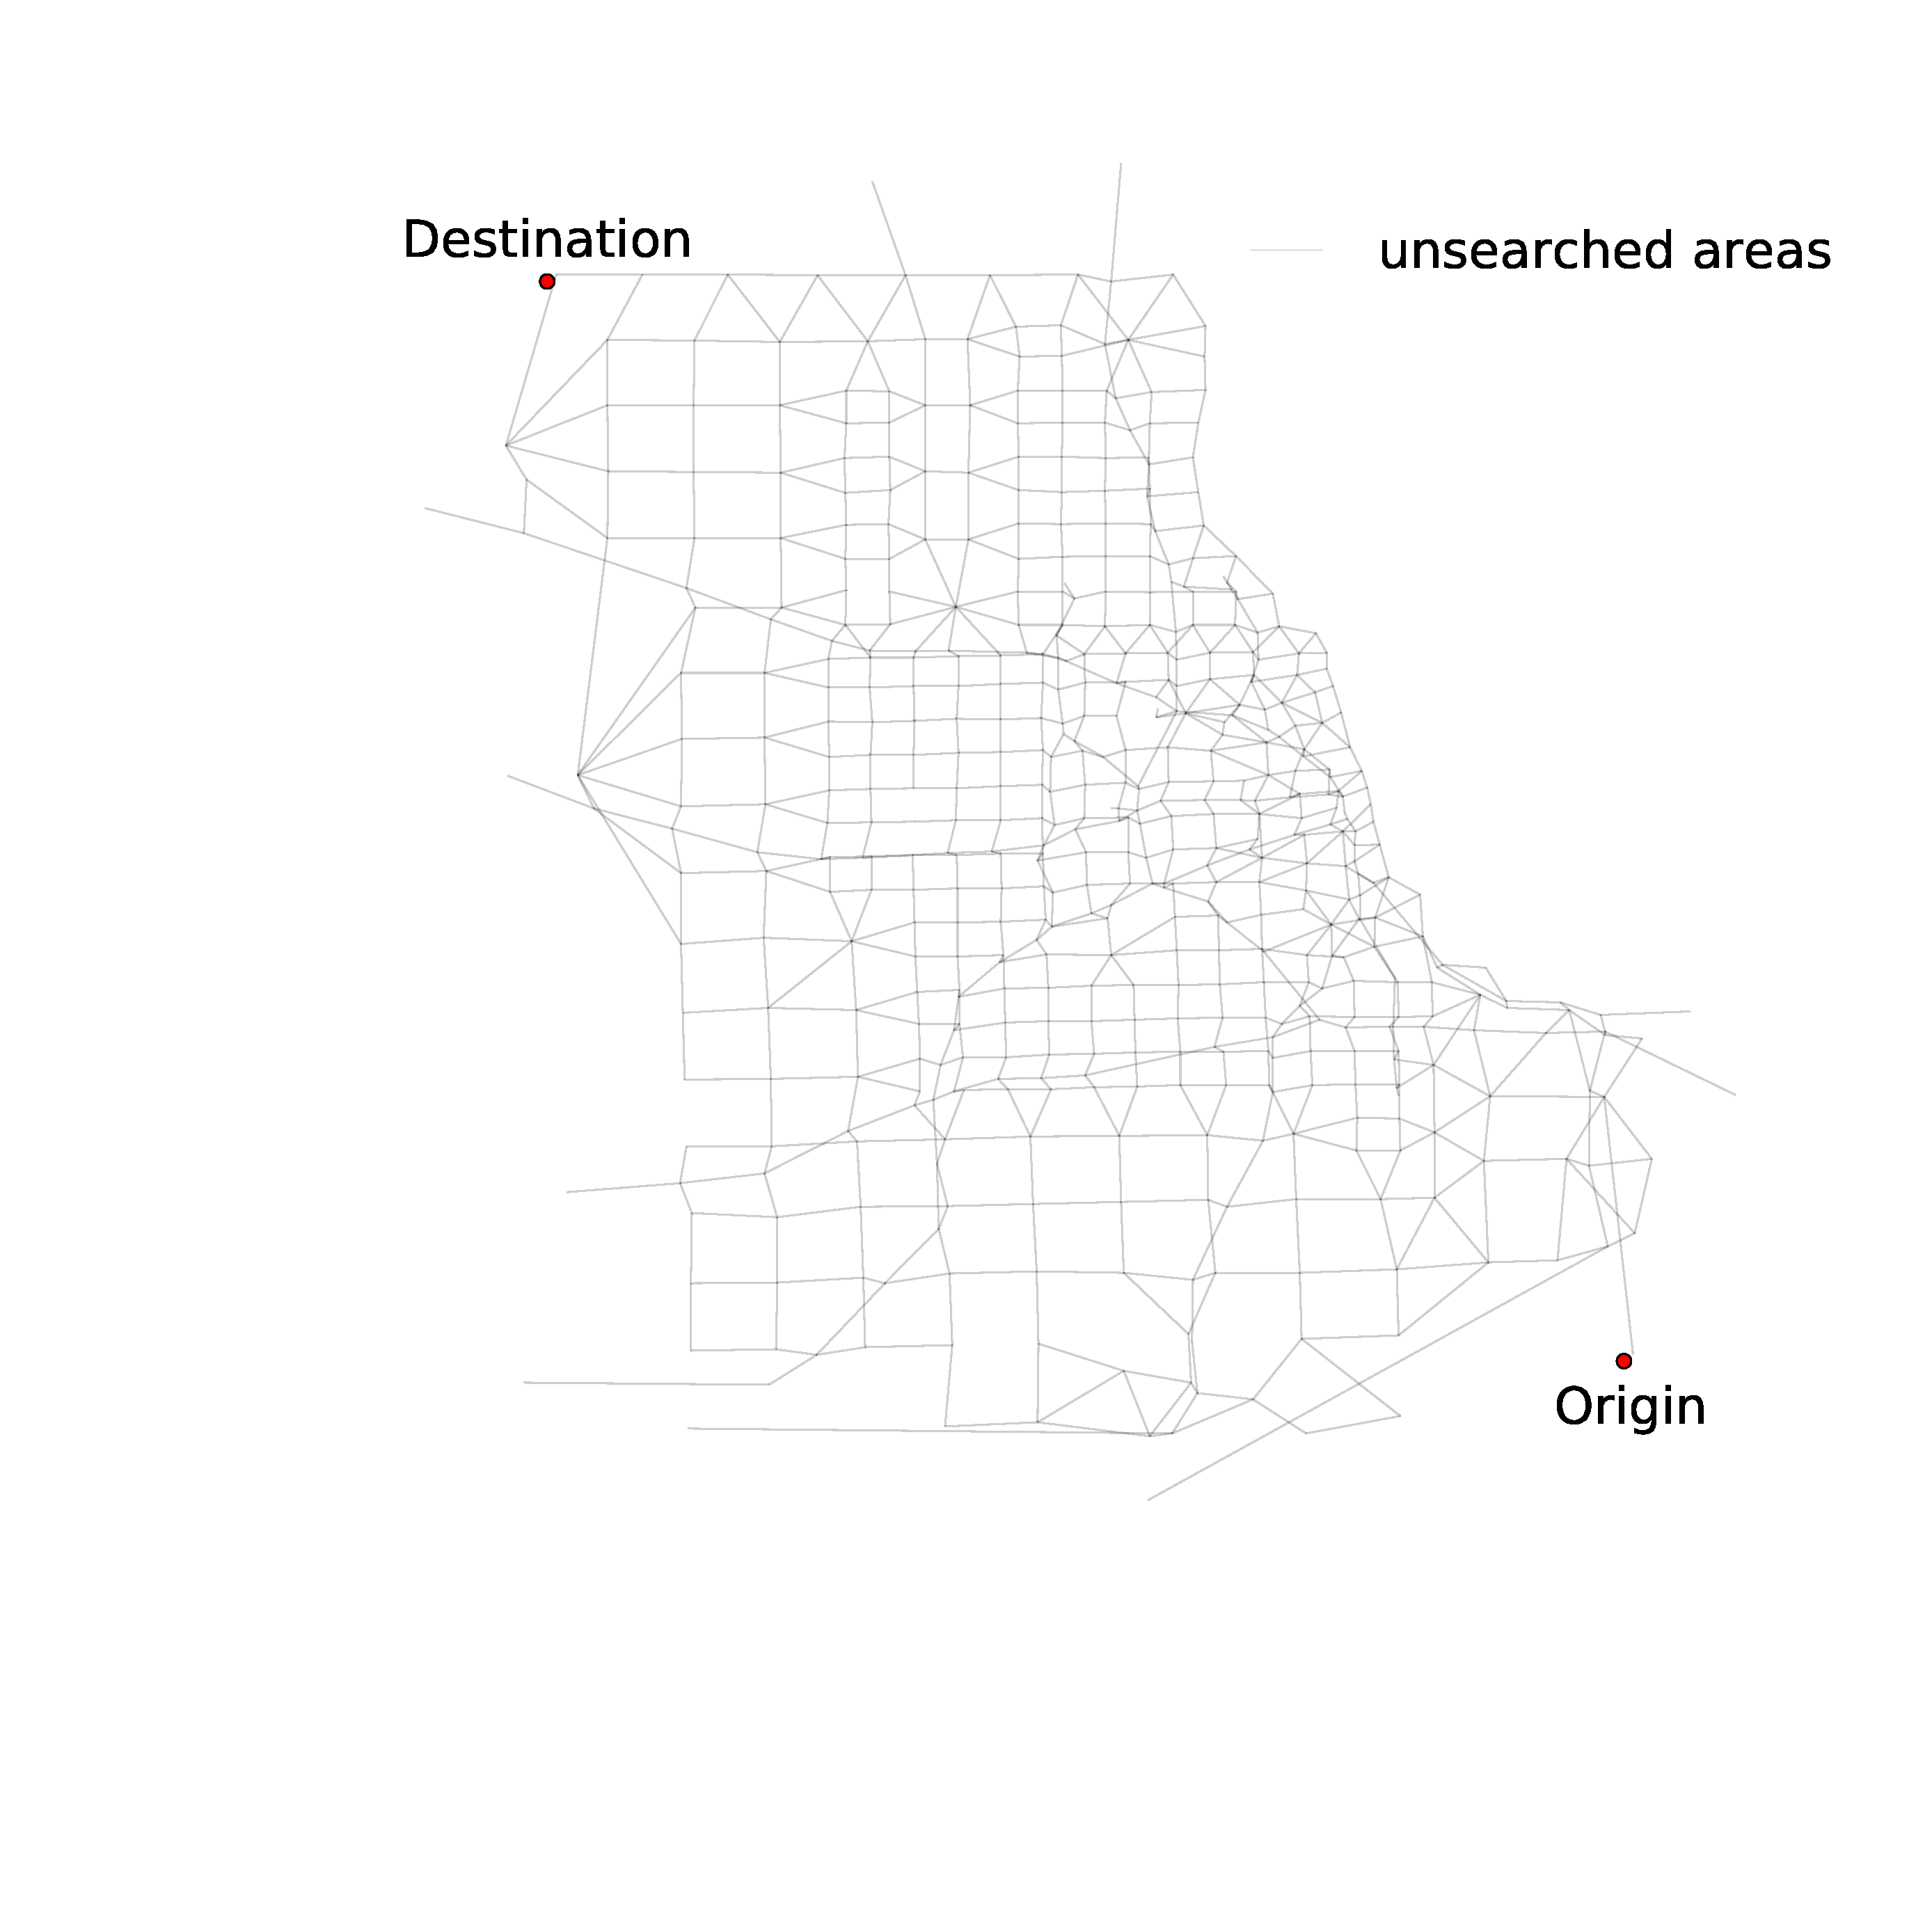
\includegraphics[page=1,width=\paperwidth, height=\paperheight, keepaspectratio,trim=0 120px 48px 120px,clip]{img/chicago_dijkstra_animation}
    \end{center}
\end{frame}

\begin{frame}[shrink]{Dijkstra's Algorithm}
    \foreach \n in {1,...,7}{
        \only<\n>{
            \begin{center}
                \includegraphics[page=\n,width=\paperwidth, height=\paperheight, keepaspectratio,trim=0 120px 48px 120px,clip]{img/chicago_dijkstra_animation}
            \end{center}
        }
    }
\end{frame}

\begin{frame}{Priority Queues Results}
    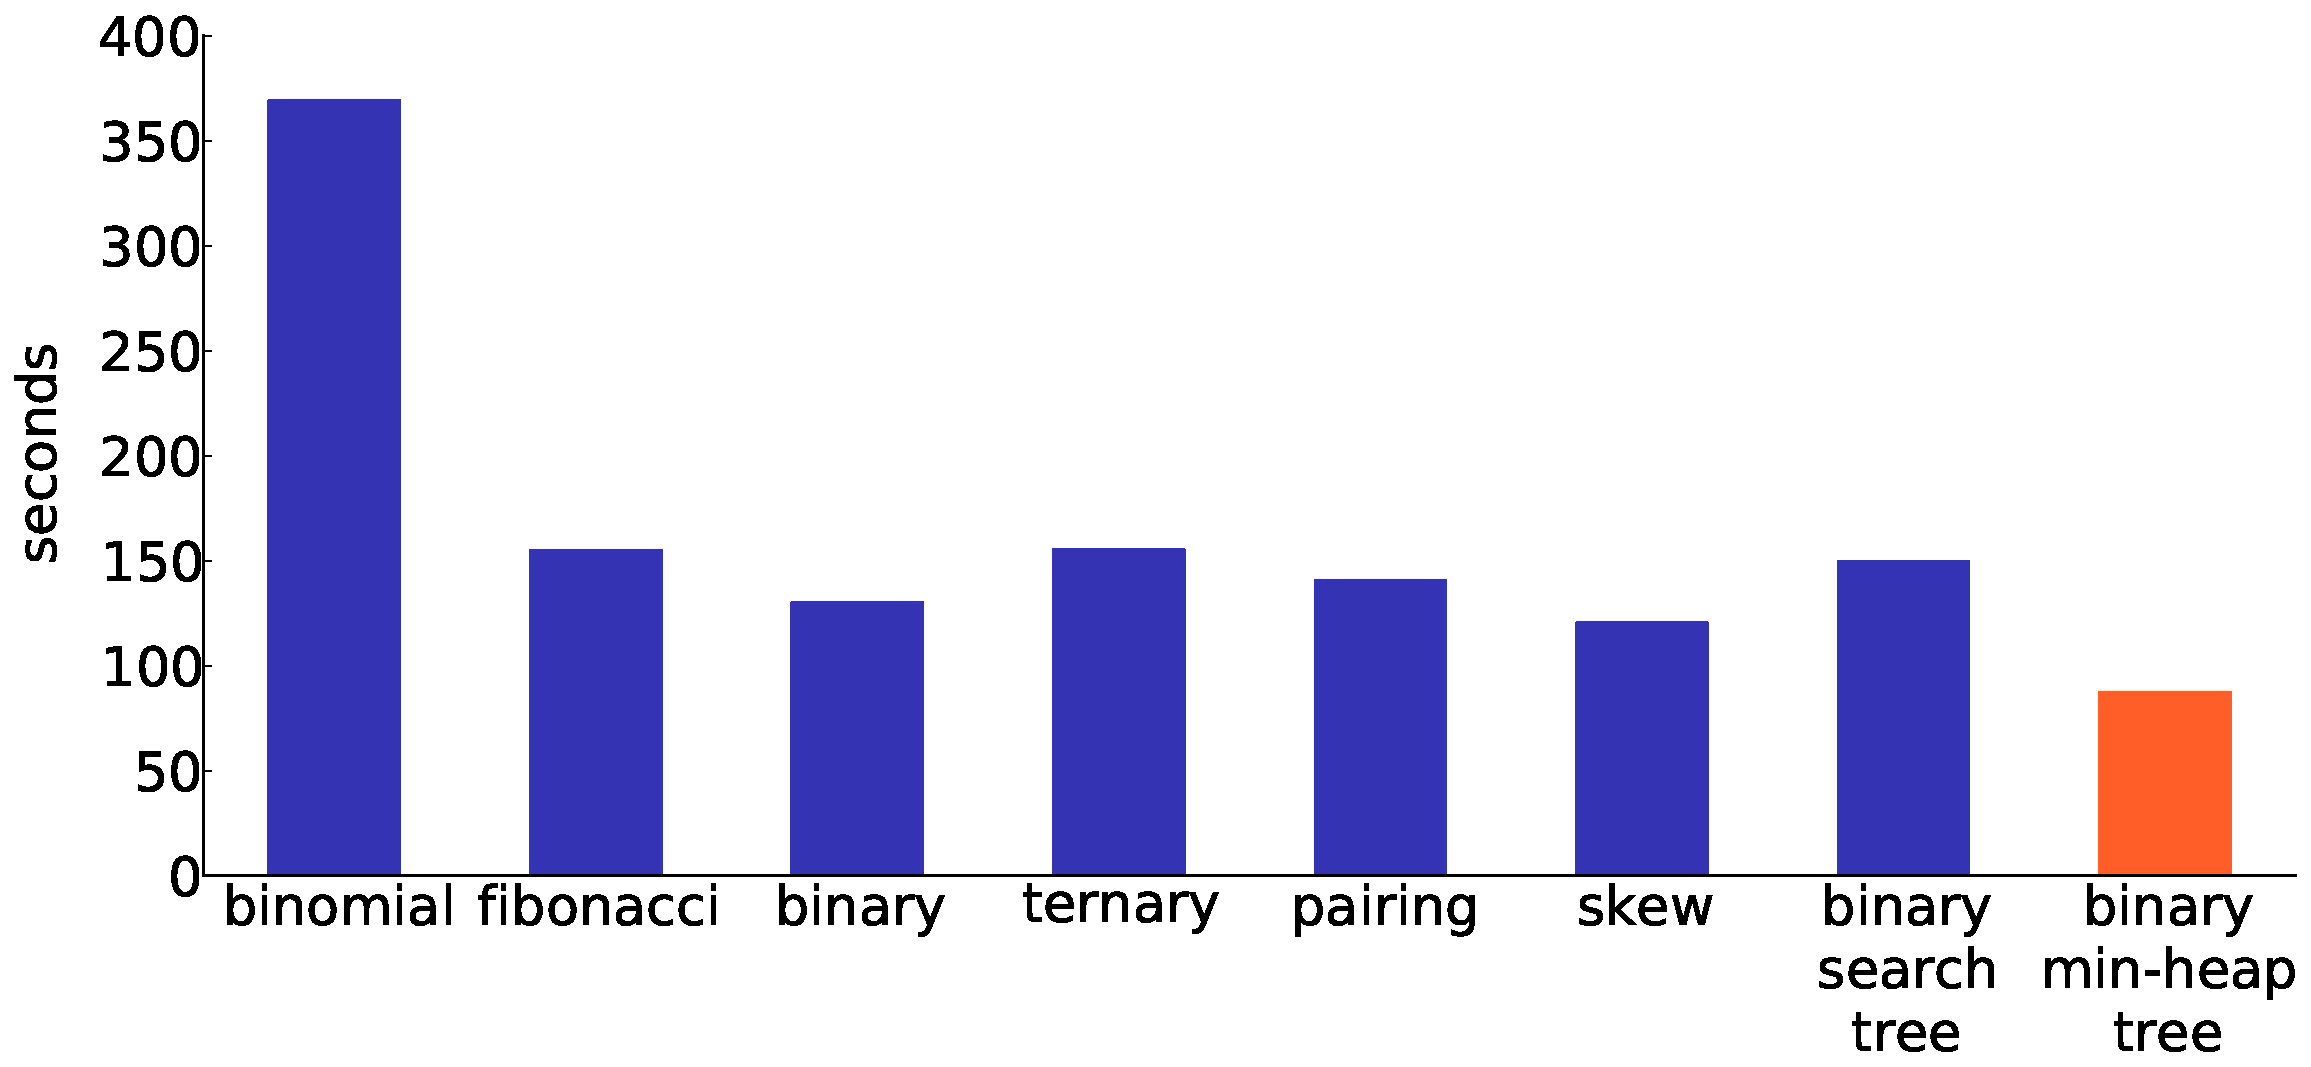
\includegraphics[width=\textwidth, keepaspectratio]{img/pq_runtime}
\end{frame}

% since we have a origin and a destination, 
% we can calculate from the two ends 
\begin{frame}[shrink]{Bidirectional Dijkstra's Algorithm}
    \foreach \n in {1,...,7}{
        \only<\n>{
            \begin{center}
                \includegraphics[page=\n,width=\paperwidth, height=\paperheight, keepaspectratio,trim=0 120px 48px 120px,clip]{img/chicago_bidirect_animation}
            \end{center}
        }
    }
\end{frame}

\begin{frame}[shrink]{A* Search (Goal-Directed Search)}
    \begin{itemize}
        \item Visit the next node that is on the expected shortest path.
    \end{itemize}
    \foreach \n in {1,...,5}{
        \only<\n>{
            \begin{center}
                \includegraphics[page=\n,width=\paperwidth, height=\paperheight, keepaspectratio,trim=0 120px 48px 120px,clip]{img/chicago_astar_animation}
            \end{center}
        }
    }
\end{frame}

\begin{frame}[shrink]{Bidirectional A* search}
    \foreach \n in {1,...,7}{
        \only<\n>{
            \begin{center}
                \includegraphics[page=\n,width=\paperwidth, height=\paperheight, keepaspectratio,trim=0 120px 48px 120px,clip]{img/chicago_astar_bidirect_animation}
            \end{center}
        }
    }
\end{frame}

\begin{frame}{Shortest Path Algorithm Results}
    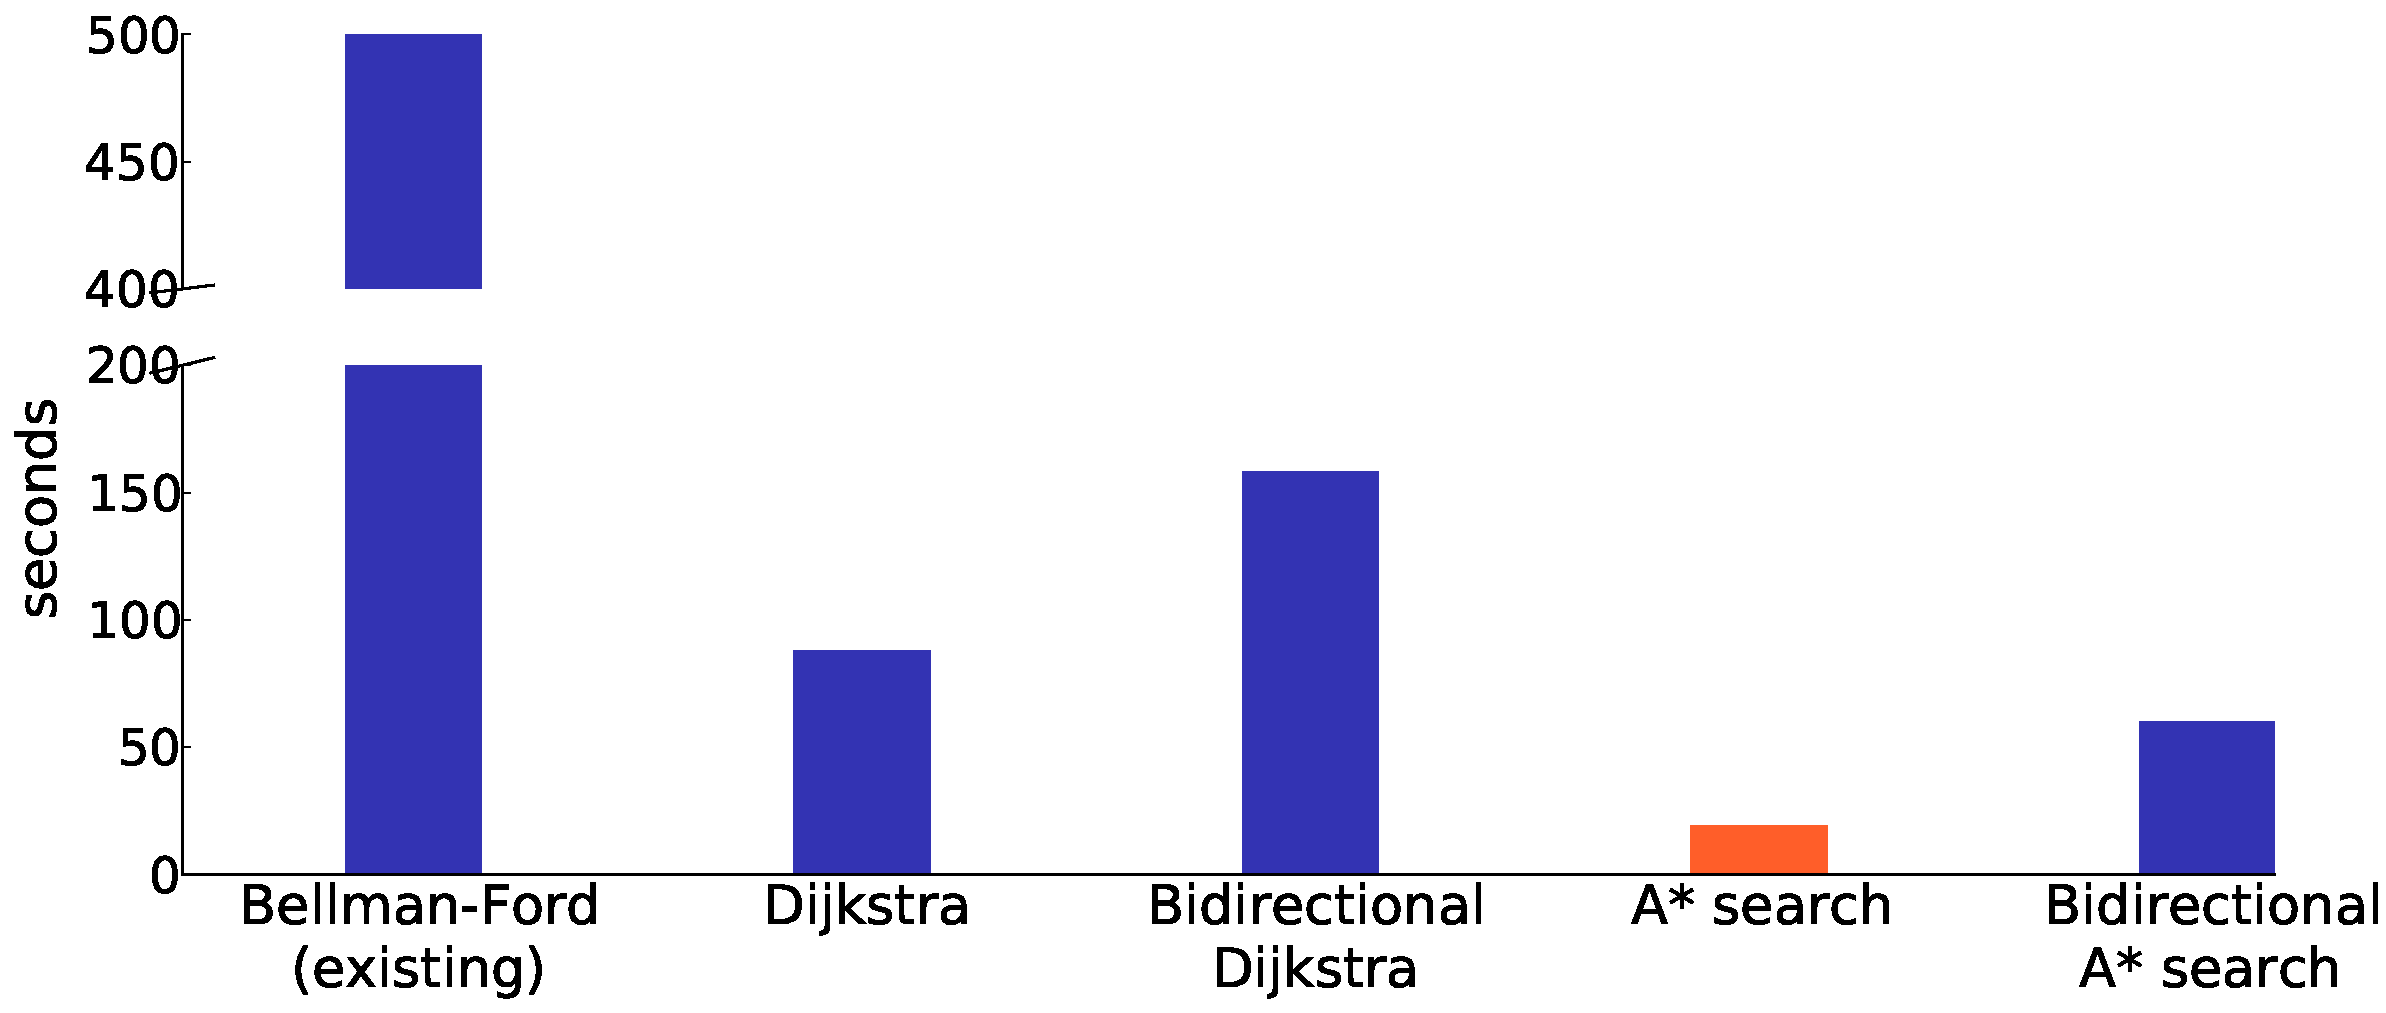
\includegraphics[width=\textwidth, keepaspectratio]{img/runtime}
\end{frame}

\begin{frame}{Avoiding shortest path calculations in traffic assignment}
    \begin{itemize}
        \item In PE, some shortest path calculations can be avoided between iterations to speed up the overall performance
        \item The shortest path from the previous iteration can be re-used to \alert{avoid} the calculation in the current iteration
    \end{itemize}
            \begin{enumerate}
                \item avoid the next few iterations if the shortest paths of the previous two iterations are identical
                \item randomly avoid the next shortest path calculation in the hope that the shortest path of previous and current iteration are identical
            \end{enumerate}
\end{frame}



\begin{frame}{Avoiding Shortest Path Calculation Results}
    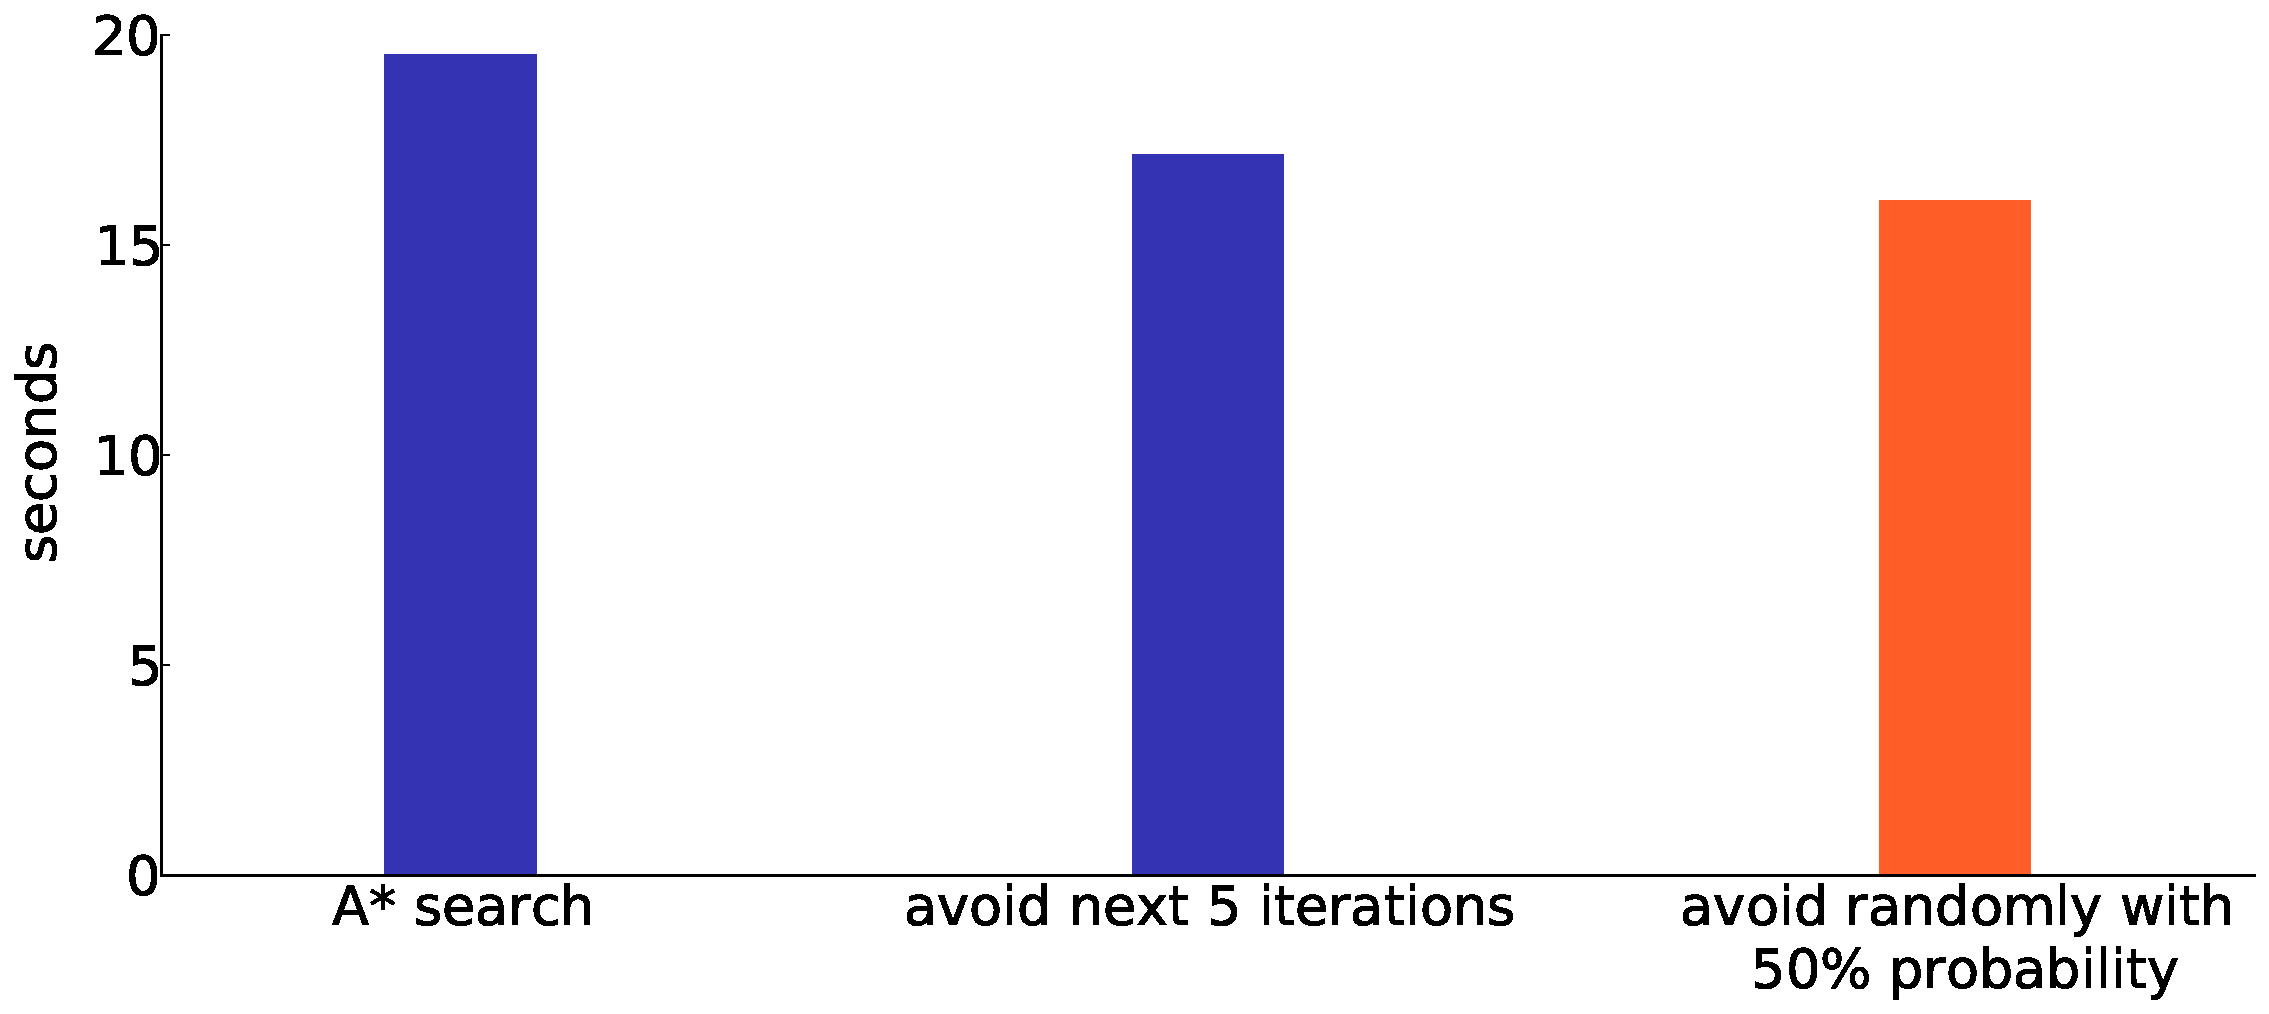
\includegraphics[width=\textwidth, keepaspectratio]{img/random_runtime}
\end{frame}

\begin{frame}{Conclusions}
    \begin{itemize}
        \item 30 times faster than the existing implemented Bellman-Ford algorithm
    \end{itemize}
\end{frame}

\begin{frame}{Future Work}
    \begin{itemize}
        \item preprocessing
            \begin{itemize}
                \item multi-thread on GPU
                \item use the avoiding strategy on similar algorithms that solve the traffic assignment problem
            \end{itemize}
    \end{itemize}
\end{frame}

\end{document}
